
\chapter{Technologie}

W rozdziale tym zaprezentowano przegl�d najwa�nieszych technologii u�ywanych do realizacji paradygmatu SOA.

\section{SOA}

Zwi�kszone zainteresowanie SOA zwi�zane jest z rozpowszechnianiem si� technologii webservice i dyskusjami na temat zysk�w, kt�re mo�na dzi�ki ich wdro�eniu osi�gn��. Problemy poruszane w tych dyskusjach nie s� nowe, pojawia�y si� ju� od czasu gdy technologia CORBA umo�liwi�a integracj� heterogenicznych aplikacji z r�nych �rodowisk. Do problem�w tych - zwi�zanych z integracj� aplikacji - mo�na zaliczy� np:

\begin{itemize}
 \item niezgodno�� danych na poziomie binarnym (np. jeden komputer u�ywa kodowania Big Endian a inny Little Endian)
 \item konieczno�� obs�ugi rozproszonych mechanizm�w transakcyjnych, autoryzacji i uwierzytelniania
 \item r�nice koncepcyjne pomi�dzy u�ytymi platformami po�rednicz�cymi (np. RMI operuje na poziomie wywo�ania metody interfejsu, Sun RPC na poziomie wywo�ania funkcji)
\end{itemize}

Technologie obiektowe stworzone w latach 90 XX wieku (CORBA, DCOM, RMI itp.) pozwalaj� na integracj� aplikacji oraz zmniejszaj� konieczno�� nadmiernego skupiania si� in�ynier�w nad kwestiami technologicznymi tego procesu. Dla przyk�adu obiekty w technologii CORBA (wykorzystuj�cej do transportu protok� IIOP) mog� komunikowa� si� nie tylko z innymi obiektami CORBA, ale tak�e np. z RMI. Technologie te nie rozwi�za�y wszystkich problem�w integracyjnych, a opr�cz nich zacz�y pojawia� si� nowe utrudnienia:

\begin{itemize}
 \item statyczno�� obiekt�w, brak mo�liwo�ci wymiany wadliwych w trakcie dzia�ania systemu
 \item �cis�e powi�zanie element�w systemu (z ang. tight coupling)
 \item redundantno�� oprogramowania (np. implementacja tej samej funkcjonalno�ci w kilku systemach)
 \item brak ponownego u�ytkowania ju� stworzonych podsystem�w
 \item integracja N podsystem�w (z kt�rych ka�dy mo�e u�ywa� ka�dego innego) wymaga�a ilo�ci po��cze� proporcjonalnej do kwadratu ilo�ci podsystem�w (por. rysunek \ref{fig:integr})
\end{itemize}

\begin{figure}[h!]
 \centering
 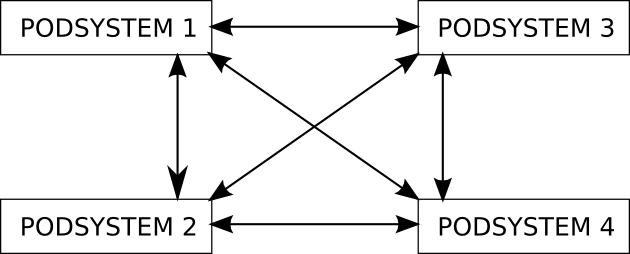
\includegraphics[bb=0 0 241 97]{chapter1/integr.png}
 % integr.png: 631x254 pixel, 188dpi, 8.51x3.43 cm, bb=0 0 241 97
 \caption{Schemat integracji 4 podsystem�w (ka�dy-z-ka�dym)}
 \label{fig:integr}
\end{figure}


Na prze�omie XX i XXI wieku pojawi�y si� technologie, kt�rych u�ycie pozwoli�o rozwi�za� cz�� wspomnianych problem�w.
Najpopularniejsze z nich to technologia webservice. Jednak opr�cz technologii potrzebny by� r�wnie� og�lny opis architektury. Architektury, w kt�rej aplikacje mog�y by� tworzone, integrowane i powt�rnie u�ytkowane; kt�ra umo�liwi�aby sk�adanie aplikacji z gotowych element�w w celu szybkiego dostarczania rozwi�za�. Pr�b� odpowiedzi na te potrzeby by�o zaproponowanie SOA.

\begin{quotation}
 \textbf{SOA} (\textbf{Service Oriented Architecture}) \cite{soa:open_group_def} - architektura zorientowana na lu�no powi�zane \textbf{us�ugi}.
\end{quotation}

\begin{quotation}
 \textbf{Us�uga} - logiczna reprezentacja powtarzalnej czynno�ci biznesowej maj�ca oczekiwany rezultat (np. pobierz prognoz� pogody, sprawd� czy osoba figuruje w krajowym rejestrze d�ug�w)\cite{soa:open_group_def}.
\end{quotation}

Podkre�lenia wymaga fakt, �e SOA i webservice nie s� poj�ciami r�wnoznacznymi. Us�ugi webservice s� dowodem i przyk�adem na istnienie technologii, kt�ra umo�liwia konstrukcj� systemu zgodnego z SOA. 
% Zostan� om�wione bardziej szczeg�owo w nast�pnym rozdziale.

Na rysunku \ref{fig:soa} znajduje si� przyk�adowy schemat funkcjonowania aplikacji opartej o SOA. Pierwszym etapem jej dzia�ania jest wyszukanie wymaganej us�ugi w rejestrze (uzyskuje si� w ten spos�b m.in. informacj� o lokalizacji us�ugi). Nast�pnie do us�ugi wys�ane zostaje ��danie wykonania operacji, kt�re jest przez ni� przetwarzane a rezultat odes�any z powrotem do aplikacji. Schemat ten jest powielany dla ka�dej z us�ug, a ca�y ci�g wywo�a� jest sterowany kodem aplikacji SOA.

\begin{figure}[h!]
 \centering
 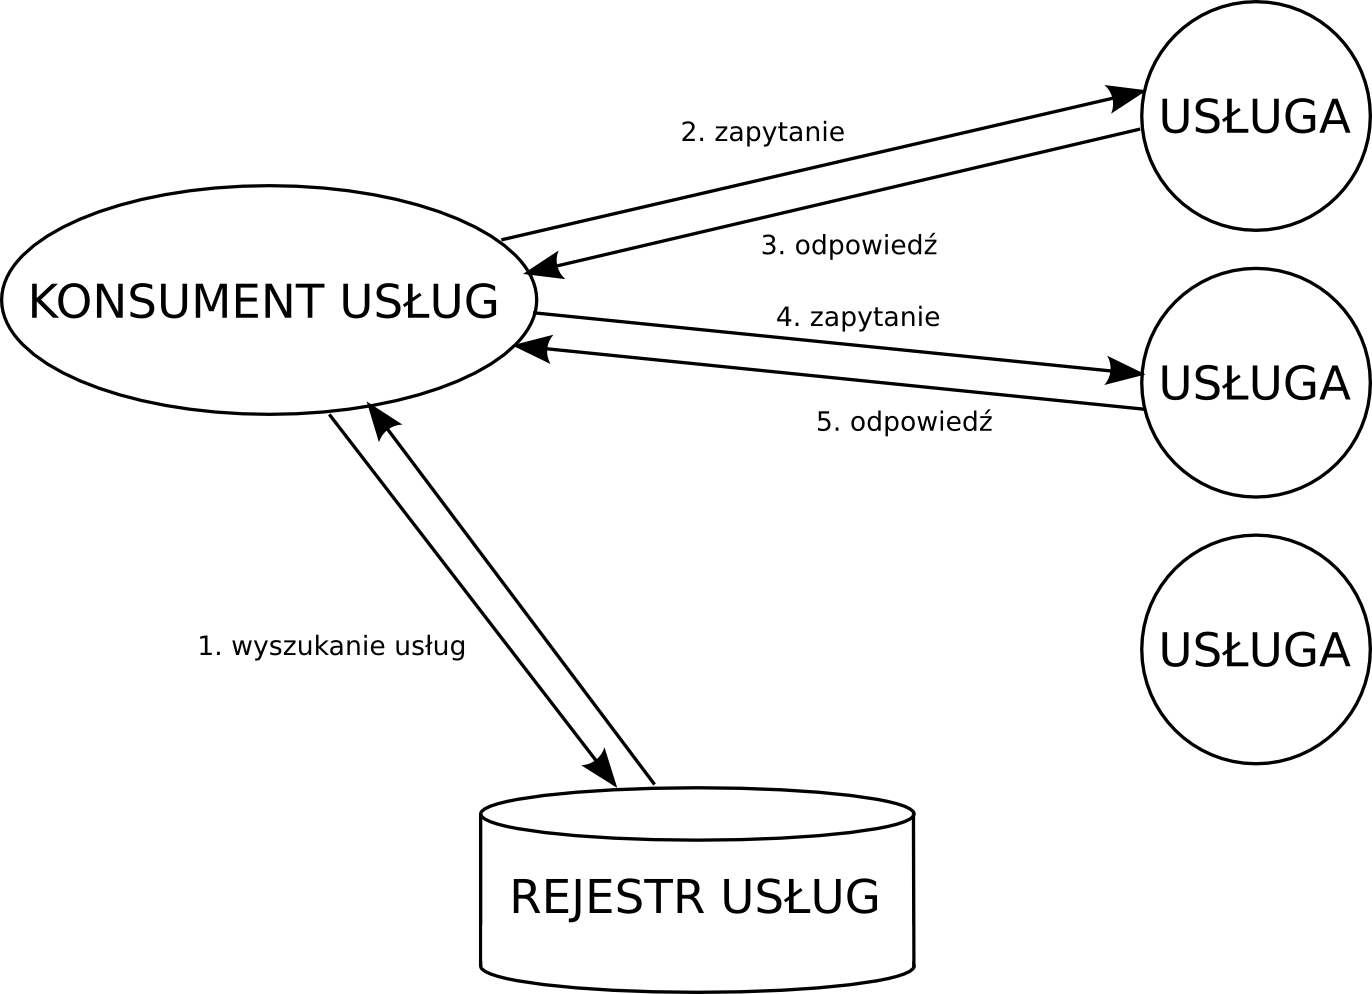
\includegraphics[bb=0 0 330 238]{chapter1/soa.png}
 % soa.png: 412x298 pixel, 90dpi, 11.63x8.41 cm, bb=0 0 330 238
 \caption{Przyk�adowy schemat funkcjonowania aplikacji opartej o SOA}
 \label{fig:soa}
\end{figure}

\subsection{Kluczowe elementy}

Wybrane elementy funkcjonowania systemu opartego o SOA:
\begin{enumerate}
 \item Wszystkie operacje systemu s� zdefiniowane jako \textbf{us�ugi}. Mog� to by� zar�wno proste operacje biznesowe (pobierz stan konta), operacje transakcyjne zbudowane z innych us�ug (przelew mi�dzy rachunkami) jak i funkcje systemowe (np. wy�lij e-mail). Do in�ynier�w nale�y decyzja o poziomie ziarnisto�ci oferowanych us�ug.
 \item Interfejs us�ugi jest \textbf{odseparowany} od implementacji. Konsumenci us�ugi nie znaj� dok�adnego sposobu realizacji operacji, znaj� jedynie semantyk� i syntaktyk� tej operacji.
 \item Prawid�owe funkcjonowanie systemu przy zachowaniu lu�nego wi�zania (ang. loose coupling) mi�dzy us�ugami uzyskuje si� dzi�ki wprowadzeniu \textbf{kontrakt�w}.
 \item System jest \textbf{systemem dynamicznym}. W trakcie jego dzia�ania mo�na dodawa� nowe us�ugi oraz wymienia� stare (np. poprawia� znalezione w nich b��dy, konstruowa� efektywniejsze wersje us�ugi).
 \item Istnieje mo�liwo�� \textbf{wielokrotnej implementacji} tej samej us�ugi w r�nych wersjach (np. za pomoc� r�nych algorytm�w, r�nych dostawc�w). U�ytkownik decyduje kt�rej instancji us�ugi chce u�y� (np. tej kt�ra w danej chwili jest najmniej obci��ona lub tej kt�ra jest najta�sza).
 \item Budowanie systemu odbywa si� na zasadzie \textbf{kompozycji} z istniej�cych ju� us�ug. Poprzednio systemy by�y tworzone poprzez integracj� element�w, co powodowa�o konieczno�� pisania kodu dostosowuj�cego mechanizmy tych element�w (np. sposobu komunikacji, obs�ugi transakcji, kontroli dost�pu).
 \item Wyst�puje ca�kowita \textbf{transparentno�� lokalizacji}. Konsument us�ugi nie jest �wiadomy gdzie fizycznie operacje danej us�ugi s� wykonywane. Us�uga mo�e w spos�b niezauwa�alny dla konsumenta migrowa� pomi�dzy maszynami w trakcie dzia�ania systemu albo by� zreplikowana na kilka maszyn w celu zmniejszenia czasu wykonywania operacji.
\end{enumerate}
Dodatkowej uwagi wymaga poj�cie kontrakt�w, b�d�cych podstaw� prawid�owej konstrukcji oprogramowania opartego o SOA.

\subsection{Kontrakt}

Kontrakty s� zawierane ka�dorazowo pomi�dzy us�ug� a jej konsumentem (kt�rym mo�e by� tak�e inna us�uga). Umo�liwiaj� separacj� interfejs�w od implementacji oraz realizacj� lu�nych powi�za� pomi�dzy us�ugami (modyfikacja szczeg��w implementacji us�ugi nie powoduje zmian w kontrakcie, a wi�c jest transparentna dla konsument�w danej us�ugi). Zawieraj� opis informacji oferowanych i oczekiwanych przez us�ug�. Dobry kontrakt powinien zawiera� nast�puj�ce pozycje \cite{soa:kontrakt}:

\begin{itemize}
 \item og�lne informacje o us�udze
   \begin{itemize}
    \item nazwa kontraktu, wersja
    \item w�a�ciciel (osoba/organizacja)
    \item rodzaj us�ugi (np. integracyjna, prezentacyjna, biznesowa)
   \end{itemize}
 \item opis funkcjonalny operacji zawartych w us�udze
   \begin{itemize}
    \item semantyka operacji (wymagania funkcjonalne w stosunku do us�ugi)
    \item syntaktyka operacji (typy argument�w i rezultat�w, wyj�tki)
    \item szczeg�y sposobu wywo�ania operacji (adres URL us�ugi oraz rodzaj protoko�u transportu np. SOAP)
   \end{itemize}
 \item opis niefunkcjonalny
   \begin{itemize}
    \item transakcyjno�� operacji
    \item QoS (Quality of Service)
    \item SLA (Service Level Agreement) np. dozwolone op�nienie w wykonywaniu us�ugi
    \item autoryzacja, ograniczenie dost�pu do operacji serwisu okre�lonej grupie konsument�w
   \end{itemize}
\end{itemize}

Podkre�lenia wymaga fakt, �e nie istnieje sformalizowana posta� kontraktu SOA. Powy�sze informacje s� jedynie proponowan� zawarto�ci� kontraktu. Rzeczywista zawarto�� kontraktu b�dzie mia�a r�n� posta� w zale�no�ci od u�ytej technologii.



\bigskip
Paradygmat SOA w praktyce mo�e zosta� zrealizowany na r�ne sposoby. Najpopularniejszym z nich jest u�ycie technologii webservice.
\section{Webservice}

Mi�dzynarodowa organizacja W3C \cite{misc:w3c} zajmuj�ca si� ustanawianiem standard�w dotycz�cych Internetu zdefiniowa�a webservice w spos�b nast�puj�cy\cite{ws:w3c_def}:

\begin{quotation}
 \textbf{Webservice} - oprogramowanie wspieraj�ce wymian� danych mi�dzy maszynami poprzez sie�, wykorzystuj�ce w tym celu zbi�r ustandaryzowanych technologii (WSDL, XML, SOAP, UDDI)\cite{ws:w3c_def}.
\end{quotation}

Webservice nie jest synonimem SOA. SOA jest to architektura zorientowana na lu�no powi�zane us�ugi, podczas gdy webservice jest to zbi�r konkretnych technologii (WSDL, XML, SOAP, UDDI), u�ytych do realizacji SOA. Technologia webservice jest wi�c przyk�adowym sposobem realizacji SOA, nie jedynym, ale w dotychczasowej praktyce jednym z najpopularniejszych.

Przyk�adowy scenariusz u�ycia webservice zaprezentowany zosta� na rysunku \ref{fig:soa-ws}. Sk�ada si� on z nast�puj�cych etap�w:
\begin{itemize}
 \item wyszukanie konkretnej us�ugi w rejestrze UDDI
 \item uzyskanie dokumentu WSDL us�ugi
 \item wys�anie zapytania zgodnego z protoko�em SOAP do us�ugi
 \item przetworzenie zapytania przez us�ug�
 \item odebranie odpowiedzi zgodnej z protoko�em SOAP od us�ugi
\end{itemize}

% przyk�ad us�ug webservice z zaznaczonymi WSDL, XML, SOAP, UDDI
\begin{figure}[h!]
 \centering
 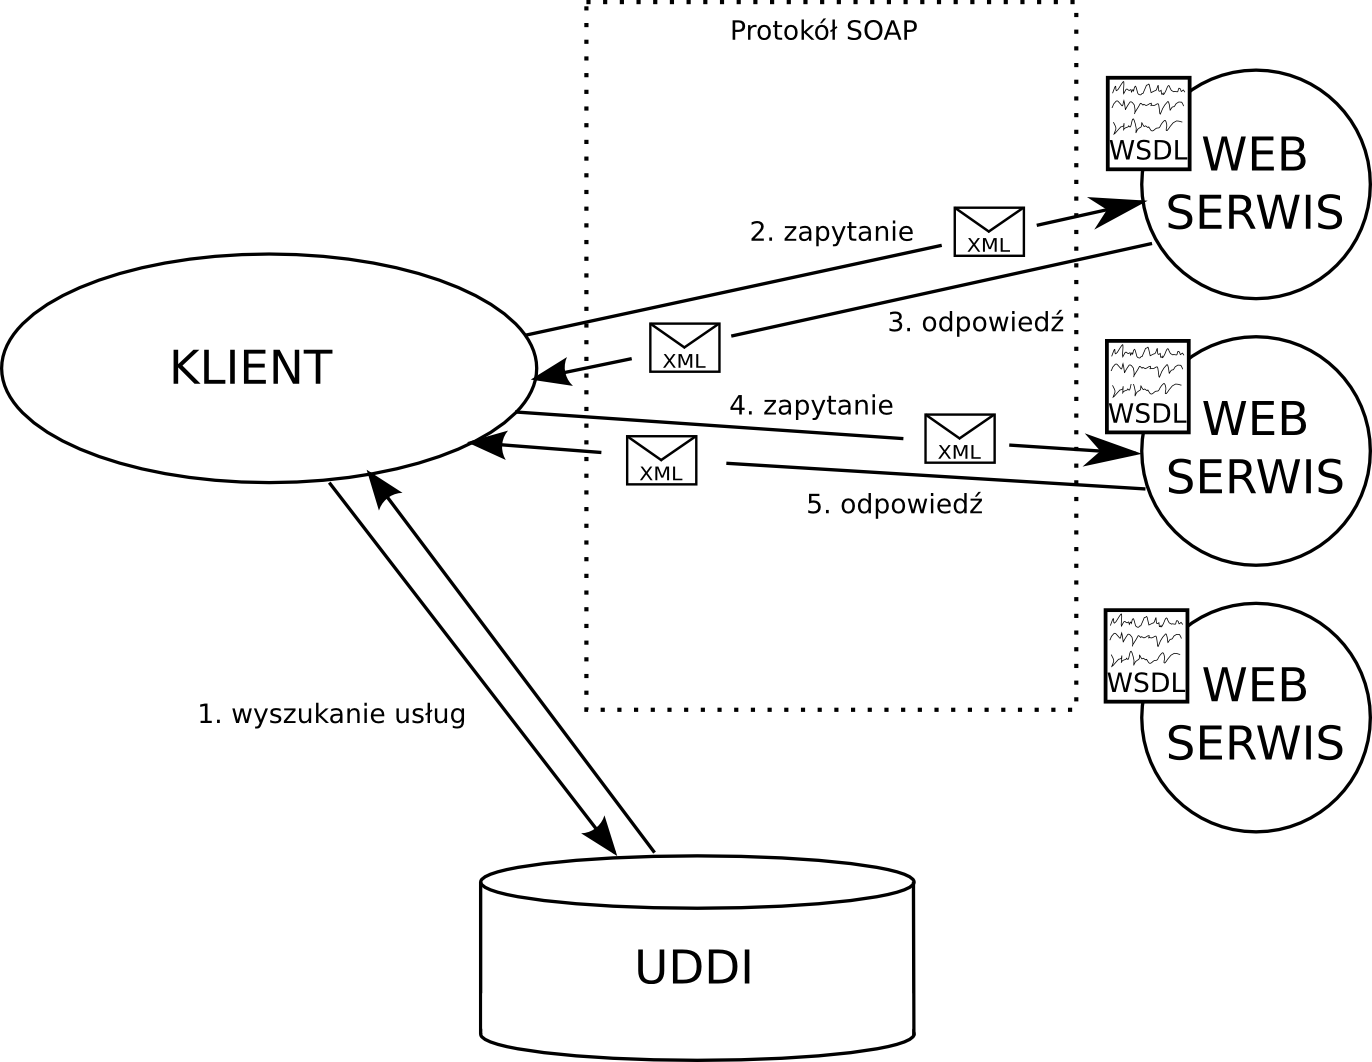
\includegraphics[bb=0 0 330 255]{chapter1/soa-ws.png}
 % soa-ws.png: 412x319 pixel, 90dpi, 11.63x9.00 cm, bb=0 0 330 255
 \caption{Przyk�ad funkcjonowania aplikacji opartej o us�ugi webservice}
 \label{fig:soa-ws}
\end{figure}

Implementacja us�ug webservice odbywa si� z wykorzystaniem ustandaryzowanych technologii:
\begin{itemize}
 \item WSDL (Web Service Definition Language) - opis us�ugi w postaci XML
 \item SOAP - protok� wymiany danych z us�ugami
 \item UDDI (Universal Description, Discovery and Integration) - obs�uga rejestru us�ug.
\end{itemize}

\subsection{WSDL}

WSDL (Web Service Definition Language) jest to dokument XML opisuj�cy webservice. Mo�e przechowywa� zar�wno og�ln� informacj� o us�udze (operacje i ich argumenty) jak r�wnie� szczeg�owe informacje (powi�zanie us�ug z protoko�ami i adresami pod kt�rymi us�ugi te s� dost�pne). Plik WSDL sk�ada si� z definicji nast�puj�cych element�w (w nawiasach podano oryginalne angielskie nazwy)\cite{ws:wsdl:spec}:
\begin{itemize}
 \item typ (type) - definicja typu danych
 \item komunikat (message) - z�o�ony typ danych
 \item operacja (operation) - definicja operacji wraz z komunikatami zawieraj�cymi argumenty oraz rezultat operacji
 \item typ portu (port type) - zbi�r operacji
 \item wi�zanie (binding) - typ portu powi�zany z konkretnym protoko�em (np. SOAP+HTTP)
 \item port (port) - wi�zanie wraz z adresem (np. URL dla HTTP, e-mail dla SMTP)
 \item us�uga (service)- zbi�r port�w
\end{itemize}

Dokument WSDL nie jest obowi�zkowym elementem ka�dego webservice. Je�li jednak wyst�puje to jest on realizacj� kontraktu SOA pomi�dzy us�ug� a jej konsumentem. Zawiera opis parametr�w oczekiwanych przez us�ug� oraz oferowanych (typ rezultatu, nazwy operacji okre�laj�ce ich semantyk�). Nie odwo�uje si� w �aden spos�b do implementacji us�ugi, dzi�ki czemu wyst�puje separacja pomi�dzy interfejsem us�ugi (opisywanym w WSDL i kontrakcie) a jej implementacj�. Zmiany w implementacji us�ugi - nie powoduj�ce zmian w semantyce ani syntaktyce operacji - nie zmieniaj� dokumentu WSDL tej us�ugi. Tym samym nie naruszaj� kontraktu i nie wymagaj� zmian u konsument�w us�ugi.

\subsection{SOAP}

SOAP (dawniej Simple Object Access Protocol, p�niej Service Oriented Architecture Protocol, obecnie brak oficjalnego rozwini�cia tego akronimu\cite{ws:w3c_soap}) jest to protok� opisuj�cy spos�b kodowania i wymiany wiadomo�ci w formacie XML. Do przesy�ania wiadomo�ci zakodowanej zgodnie z SOAP najcz�ciej wykorzystuje si� protok� HTTP/HTTPS (ze wzgl�du na jego popularno�� w internecie), ale mo�liwe jest te� wykorzystanie np. SMTP, FTP, RMI/IIOP. Protok� SOAP mo�e by� u�yty w realizacji r�nych wzorc�w wymiany wiadomo�ci (MEP - Message Exchange Pattern), ale dla potrzeb webservice u�ywa si� go w RPC (RPC - Remote Procedure Call)\cite{ws:w3c_soap_rpc}.

Wiadomo�� SOAP z za��cznikami sk�ada si� z:
\begin{itemize}
 \item w�a�ciwej wiadomo�ci SOAP w formacie XML
  \begin{itemize}
   \item element�w nag��wka (opcjonalne)
   \item tre�ci wiadomo�ci
  \end{itemize}
 \item za��cznik�w przechowuj�cych dane binarne
\end{itemize}

\begin{figure}[h!]
 \centering
 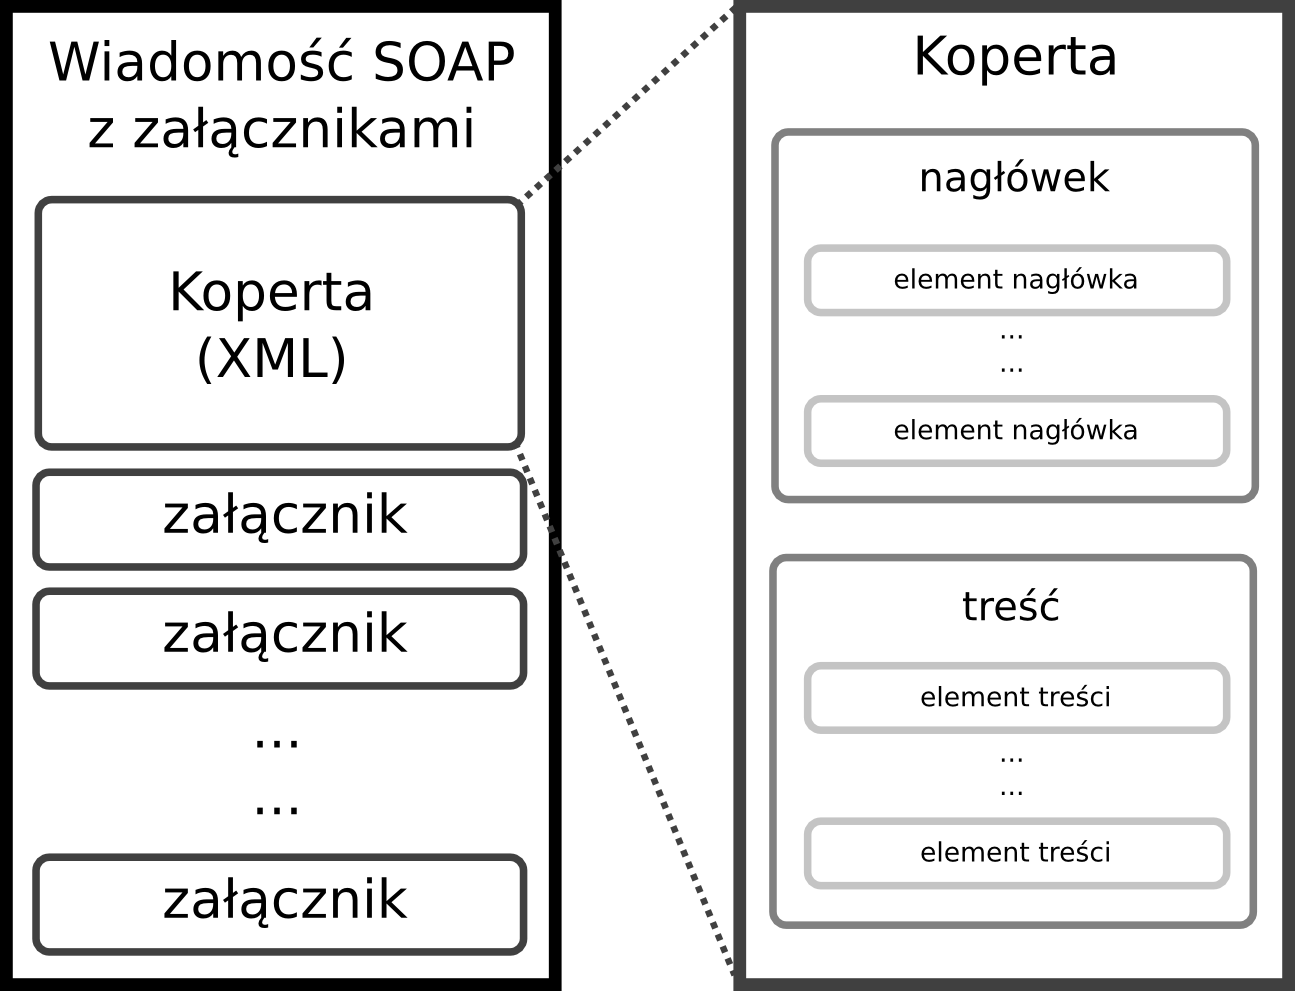
\includegraphics[bb=0 0 311 238]{chapter1/soap.png}
 % soap.png: 1295x991 pixel, 300dpi, 10.96x8.39 cm, bb=0 0 311 238
 \caption{Posta� wiadomo�ci SOAP z za��cznikami \cite{ws:suntechdays}}
 \label{fig:soap}
\end{figure}

Proces wykonania operacji danego webservice rozpoczyna si� od stworzenia odpowiedniej wiadomo�ci w formacie SOAP. Format tej wiadomo�ci zosta� przedstawiony na rysunku \ref{fig:soap}. W jej tre�ci przesy�ane s� informacje o ��danej operacji oraz warto�ciach jej parametr�w. Dodatkowo (w nag��wku) mog� by� przekazane np. parametry do autoryzacji (nazwa u�ytkownika i has�o), identyfikator sesji. Po wys�aniu wiadomo�ci do us�ugi (np. na adres uzyskany z pliku WSDL) nast�puje wykonanie ��danej operacji i odes�anie odpowiedzi do nadawcy. Odpowied� jest r�wnie� zakodowana w formacie SOAP i zawiera informacje o rezultacie wykonania operacji (lub ewentualnych wyj�tkach).

\subsection{UDDI}
UDDI (Universal Description, Discovery and Integration)\cite{ws:uddi} - technologia pozwalaj�ca na publikacj� i wyszukiwanie informacji o us�ugach webservice. Jest to otwarty standard zarz�dzany przez organizacj� OASIS \cite{ws:oasis}. Spos�b wykorzystania UDDI opiera si� na mechanizmie publikacja-wyszukanie-powi�zanie (z ang. publish-find-bind) przedstawionym na \nolinebreak{rysunku \ref{fig:uddi}}:
\begin{itemize}
 \item u�ycie us�ugi musi by� poprzedzone \textbf{opublikowaniem} jej w rejestrze
 \item konsument \textbf{wyszukuje} interesuj�ce go us�ugi w rejestrze
 \item po znalezieniu us�ugi nast�puje \textbf{powi�zanie} jej z konsumentem, kt�ry uzyskuje mo�liwo�� wykonywania operacji tej us�ugi
\end{itemize}


\begin{figure}[h!]
 \centering
 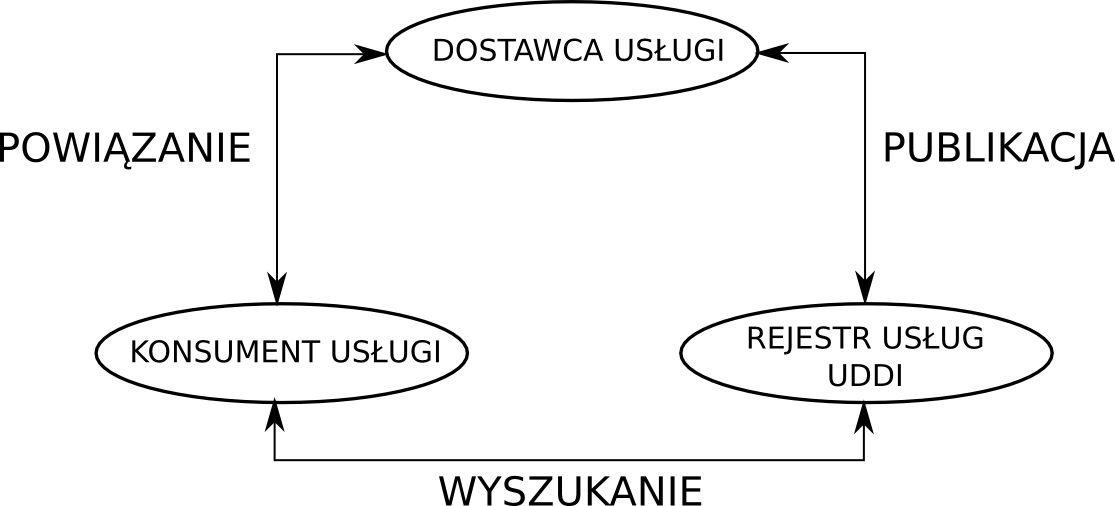
\includegraphics[bb=0 0 268 122]{chapter1/uddi.png}
 % uddi.png: 700x318 pixel, 188dpi, 9.44x4.29 cm, ABB=0 0 268 122
 \caption{Schemat wykorzystania UDDI \cite{ws:suntechdays}}
 \label{fig:uddi}
\end{figure}

UDDI przechowuje informacj� o zbiorze podmiot�w biznesowych. Pojedy�czy wpis o podmiocie biznesowym podzielony jest na nast�puj�ce grupy:
\begin{itemize}
 \item ``white pages'' - adres, dane kontaktowe
 \item ``yellow pages'' - kategorie do jakich nale�y biznes i jego us�ugi
 \item ``green pages'' - techniczne informacje o udost�pnianych us�ugach (m.in. adresy URL plik�w WSDL)
\end{itemize}

W roku 2000 wraz ze specyfikacj� standardu UDDI powsta� publiczny rejestr us�ug UDDI stworzony przez firm� IBM, Microsoft oraz SAP \cite{ws:uddi:public}. 
%Rejestr ten zosta� wy��czony w roku 2006 i do tego czasu 
W rejestrze tym, do momentu jego wy��czenia w roku 2006, zgromadzono ponad 50000 wpis�w o us�ugach \cite{ws:uddi:public}. Wy��czenie publicznego rejestru by�o efektem zwi�kszaj�cego si� zainteresowania podmiot�w biznesowych prywatnymi rejestrami UDDI.


\bigskip
Opr�cz technologii webservice mo�liwo�� realizacji paradygmatu SOA daje r�wnie� platforma integracyjna ESB.
\section[ESB]{Enterprise Service Bus}

% 
ESB (Enterprise Service Bus) to jedno z podej�� kt�re u�atwia tworzenie oprogramowania o architekturze SOA. Zak�ada ono tworzenie sterowanego zdarzeniami systemu opartego o lu�no powi�zane us�ugi. Wymiana danych jest dokonywana przez szyn�,
 kt�rej zadaniem jest wyznaczanie tras wiadomo�ci, na podstawie dostarczonej konfiguracji. G��wnym zamiarem jej tw�rc�w by�o rozlu�nienie powi�zania pomi�dzy wykorzystywanymi us�ugami, a medium transportowym, co przedstawia rysunek \ref{fig:esb}. 
 
% Jest to oparta na standardach platforma integracyjna, kt�ra
% ��czy w sobie zalety takich podej�� jak komunikacja w oparciu o wiadomo�ci, technologia WebService, transformacje danych, inteligentne wyznaczanie trasy, niezawodno��, orchiestracja i transakcyjno�� w komunikacji pomi�dzy r�norodnymi
% aplikacjami korporacyjnymi\footnote{z ang. \textit{enterprise applications}}.
% Ca�a idea opiera si� na istnieniu szyny, w oparciu o kt�r� odbywa si� ka�da komunikacja w obr�bie tworzonego systemu. Odpowiednio skonfigurowana - jest w stanie sama decydowa� o przeznaczeniu ka�dej wiadomo�ci, na podstawie jej tre�ci\footnote{z ang. content based routing}.
% Skonfigurowana szyna decyduje o tym gdzie ma zosta� wys�ana przetwarzana wiadomo��.
% Dzi�ki swoim w�a�ciwo�ciom szyna jest w stanie sama
% decydowa� o tym gdzie ma wys�a� dan� wiadomo��. % napisa� o tym �e to my decydujemy o tym jak lataj� wiadomo�ci

%\begin{figure}[htb!]
% \centering
% 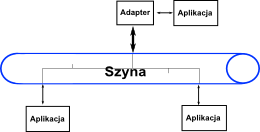
\includegraphics[bb=0 0 208 106]{chapter1/esb.png}
% % esb.png: 260x132 pixel, 90dpi, 7.34x3.73 cm, bb=0 0 208 106
% \caption{Zasada dzia�ania ESB \cite{esb:sojbi}}
% \label{fig:esb}
%\end{figure}

\begin{figure}[htb!]
 \centering
 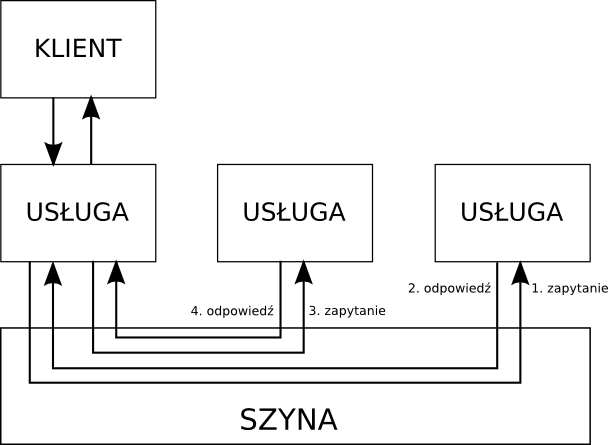
\includegraphics[bb=0 0 233 170]{chapter1/esb2.png}
 % esb2.png: 608x445 pixel, 188dpi, 8.21x6.01 cm, bb=0 0 233 170
 \caption{Zasada dzia�ania ESB \cite{esb:sojbi}}
 \label{fig:esb}
\end{figure}


\subsection{Historia ESB}
ESB powsta�o na bazie scharakteryzowanych poni�ej, bardzo obecnie popularnych koncepcji MOM i EAI. 
% Poni�ej znajduje si� ich kr�tka charakterystyka.

% Na kszta�t ESB mia�o wp�yw wiele do�wiadcze� z wcze�niejszych pr�b kompleksowego podej�cia 
% do problemu integracji us�ug. Najbardziej znacz�cy wk�ad mia�y koncepcje MOM oraz EAI:

\paragraph{Message Oriented Middleware}
to architektura kt�rej rozw�j rozpocz�� si� na pocz�tku lat 80 i trwa do dzi�. Opiera si� ona na koncepcji asynchronicznej wymiany jednostek danych (wiadomo�ci) za pomoc� jednolitych protoko��w komunikacyjnych. % zastanowi� si� czy jednolitych i czy wiadomo�ci czy komunikaty
Podstawowymi trybami komunikacji MOM s�: % bo mog� by� inne
\begin{itemize}
\item  Point-to-Point (punkt-punkt) - tryb w kt�rym istnieje tylko jeden
producent i jeden konsument wiadomo�ci
\item  Publish/Subscribe (publikuj/zapisz si�) - tryb w kt�rym istnieje jeden
producent, a odbiorc�w mo�e by� dowolna ilo��.
\end{itemize}

U�ycie rozwi�za� MOM sta�o si� standardem obs�ugi asynchronicznych zdarze� w du�ych aplikacjach biznesowych, stymuluj�c jednocze�nie ich rozw�j. Wiele z nich posiada tak zaawansowane w�a�ciwo�ci jak: niezawodno�� dostarczania, kolejkowanie i filtrowanie wiadomo�ci, transakcyjno��, mo�liwo�� klastrowania, czy zaawansowane mechanizmy bezpiecze�stwa. 

Do standard�w realizuj�cych ide� MOM nale�� mi�dzy innymi:JMS (Java Messaging System) \cite{esb:mom:jms}, IceStorm \cite{esb:mom:icestorm}, CORBA Notification Service \cite{esb:mom:corba}, Microsoft MSQM \cite{esb:mom:msqm} oraz specyfikacje WS-Events \cite{esb:mom:wsevents} i WS-Notifications \cite{esb:mom:wsnotifications}.

\begin{figure}[h!tb]
 \centering
 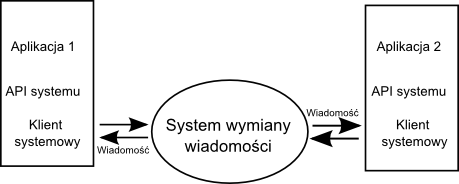
\includegraphics[bb=0 0 221 88]{chapter1/mom.png}
 % mom.png: 273x109 pixel, 89dpi, 7.79x3.11 cm, bb=0 0 221 88
 %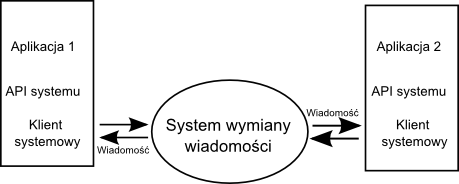
\includegraphics[bb=0 0 203 88]{chapter1/mom.png}
 %% mom.png: 251x109 pixel, 89dpi, 7.16x3.11 cm, bb=0 0 203 88
 \caption{Zasada dzia�ania MOM}
 \label{fig:mom}
\end{figure}


% Dzi�ki du�ej popularno�ci rozwi�za� typu MOM, wiele doczeka�o si� w�a�ciwo�ci
% kt�re powoduj�, �e s� one z powodzeniem wykorzystywane w aplikacjach o du�ych wymaganiach - takich jak:
% nie jest to po polsku
% du�a popularno�� rozw. MOM zaowocowa�a ich dalszym rozwojem i wzbogacaniem o nowe wlasciwosci!!!

% \begin{itemize}
% \item  \textbf{niezawodno�� dostarczania wiadomo�ci} zapewniana przez za�o�enie,
% ka�da wiadomo�� jest autonomiczna (tj. w momencie jej wys�ania rola aplikacji w
% przetwarzaniu danego elementu ko�czy si�) oraz przez zastosowanie:
% \begin{itemize}
% \item  kolejkowania i zapewnienia dostarczenia, tzw. mechanizm
% store-and-forward, kt�ry powoduje, �e wiadomo�� dociera do adresata nawet je�li
% do��czy on do kana�u informacyjnego dopiero po jakim� czasie od wys�ania
% wiadomo�ci \footnote{du�e znaczenie ma tutaj tzw. persystencja wiadomo�ci celem
% jej dalszego u�ycia}
% \item  mechanizm�w potwierdze� pozwalaj�cych wysy�aj�cemu upewni� si�, �e
% wiadomo�� dotar�a do adresata
% \end{itemize}
% 
% \item \textbf{filtrowanie wiadomo�ci} na podstawie p�l nag��wka
% 
% \item \textbf{hierarchiczno�� temat�w} mechanizmu publish/subscribe - polega na
% tym �e wiadomo�ci
% wysy�ane do temat�w nadrz�dnych trafiaj� do jego wszystkich podga��zi
% \item \textbf{mechanizmy autoryzacji} wysy�ania i odbierania wiadomo�ci w
% oparciu o ACL z uwzgl�dnieniem hierarchi temat�w
% \item \textbf{obs�uga transakcyjno�ci} tzn. dostarczanie wiadomo�ci jest
% % co z t� transakcyjno�ci� 
% zablokowane do czasu, a� transakcja zostanie zako�czone oraz wszystkie
% wiadomo�ci zostan� pomy�lnie wys�ane 
% \end{itemize}

% napisac o dodatkowych wlasciwosciach niefunkcjonalnych tak jak load-balancing, fail-over...

\paragraph{EAI}
Enterprise Application Integration, to idea kt�ra pojawi�a si� w po�owie lat 90. Celem jaki przy�wieca� jej tw�rcom by�a redukcja ilo�ci koniecznych po��cze�
w systemie rozproszonym poprzez wprowadzenie jednego centralnego punktu tzw. hub-and-spoke broker (pol. po�rednik w strukturze gwia�dzistej). Na punkcie tym spoczywa zadanie zawiadywania ca�� komunikacj� w obr�bie systemu - to on decyduje o tym gdzie ma trafi� dana wiadomo��. Architektura ta separuje aplikacj� od w�a�ciwego kodu integruj�cego poprzez u�ycie oprogramowania BPM (Business Process Management)\cite{esb:bpm}.
\begin{figure}[h!tb]
 \centering
 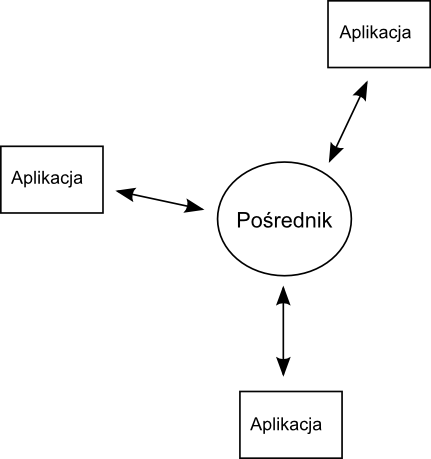
\includegraphics[bb=0 0 207 221]{chapter1/eai.png}
 % eai.png: 256x273 pixel, 89dpi, 7.31x7.79 cm, bb=0 0 207 221
 \caption{Zasada dzia�ania EAI \cite{esb:book:chapell}}
 \label{fig:eai}
\end{figure}

W za�o�eniach EAI mia�a by� stosowana w nast�puj�cych przypadkach:
\begin{itemize}
 \item Integracja proces�w biznesowych - zapewnienie ��czno�ci pomi�dzy
 procesami biznesowymi aplikacji istniej�cych w du�ych systemach
 \item Zapewnianie integralno�ci danych w r�nych cz�ciach systemu\footnote{Znane r�wnie� pod terminem EII (Enterprise Information
 	 Integration)}
 \item Uniezale�nienie implementacji od system�w zewn�trznych - przeniesienie 
 regu� i polityk biznesowych do EAI, tak aby zmiany dostawc�w nie wp�ywa�y na
  inne cz�ci
 systemu
 \item Udost�pnienie ujednoliconego interfejsu dla z�o�onych aplikacji
\end{itemize}

Istnieje wiele implementacji EAI, w�r�d najbardziej znanych znajduj� si�:
Microsoft BizTalk Server\texttrademark, SAP Exchange Infrastructure (SAP XI) \texttrademark oraz webMethods Integration Server \texttrademark.

% \subsection{ESB jako potomek MOM i EAI}
% ESB jako koncepcja maj�ca swe podwaliny w obu tych podej�ciach. Z MoM zaczerpn�a komunikacj� w oparciu o rozproszon� infrastruktur�, oddzielaj�c jednocze�nie mechanizm regu� systemowych (biznesowych) od implementacji poszczeg�lnych cz�ci systemu:

\paragraph{ESB jest pochodn� obu technologii}

\begin{figure}[h!tb]
 \centering
 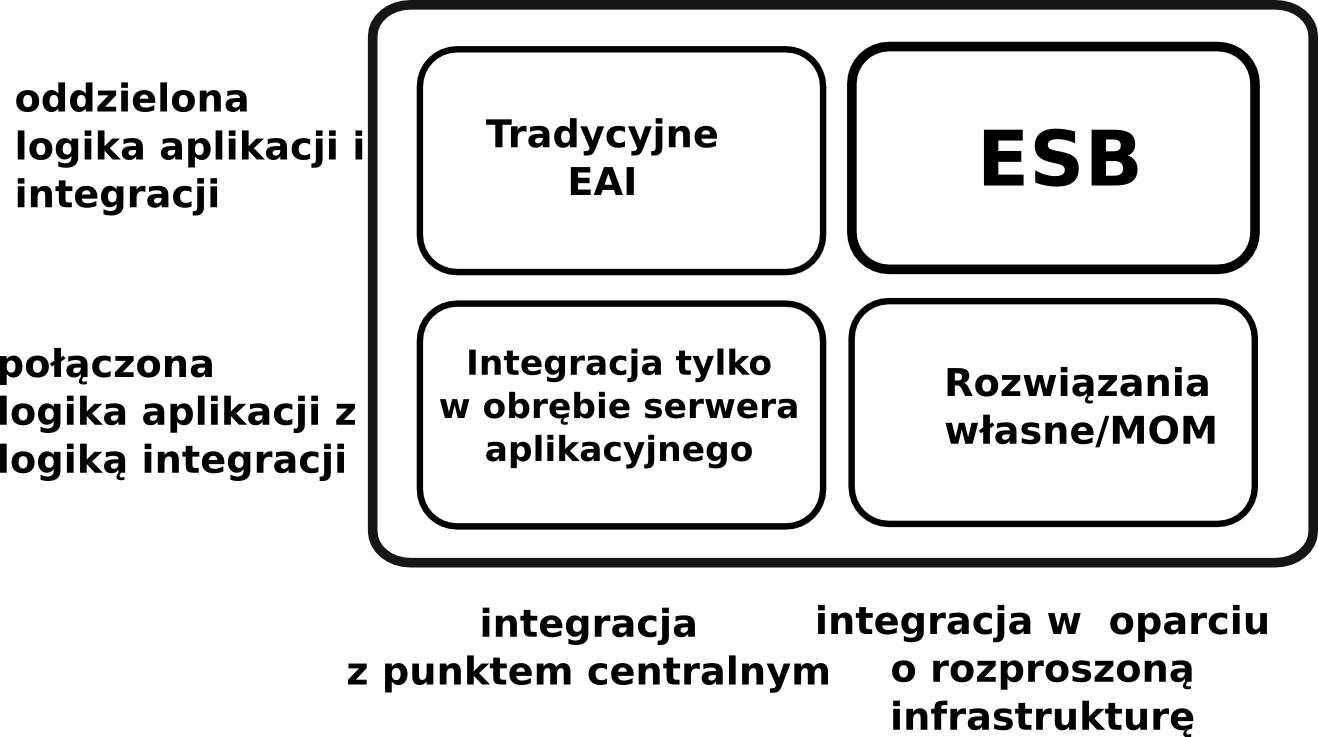
\includegraphics[bb=0 0 317 177]{chapter1/esb-where.png}
 % esb-where.png: 1318x737 pixel, 300dpi, 11.17x6.24 cm, bb=0 0 317 177
 \label{fig:esb_where}
 \caption{ESB jako pochodna EAI i MOM}
\end{figure}

Rysunek \ref{fig:esb_where} obrazuje spos�b w jaki ESB czerpa�o swoje cechy z obu podej��. Korzysta z charakterystycznej dla MOM rozproszonej infrastruktury dostarczania wiadomo�ci oraz oddziela logik� dostarczania od ich w�a�ciwego przetwarzania, co jest specyficzne dla EAI.

\subsection{Za�o�enia i cechy ESB}

Jednym z najwa�niejszych zamierze� tw�rc�w ESB by�o osi�gniecie mo�liwo�ci zastosowania tego rozwi�zania w najwi�kszej liczbie przypadk�w. Dlatego te� idea ESB opiera si� na nast�puj�cych za�o�eniach:
\begin{itemize}
	\item adaptowalno�� niezale�na od warunk�w wdro�enia - skali,
 technologii uczestnicz�cych czy sposobu modelowania aplikacji
	\item zunifikowane podej�cie do po��czenia poszczeg�lnych element�w 
oprogramowania
	\item �atwo�� integracji z oprogramowaniem zar�wno wewn�trz, jak i na 
zewn�trz korporacji
	\item prostota tworzenia aplikacji i dodawania do ju� istniej�cego
	 rozwi�zania
	\item zdecentralizowanie dzia�ania us�ug integracyjnych
	\item zwi�kszona przejrzysto�� systemu
	\item du�a elastyczno�� i �atwo�� reagowania na zmieniaj�ce si�
	wymagania
	\item zapewnienie du�ej skalowalno�ci tworzonych rozwi�za�.
\end{itemize}

% nie ma tu co napisac na koncu

\paragraph{Cechy ESB}
Z uwagi na fakt, i� koncepcja ESB nie jest poparta �adnym standardem, nie da si� wyr�ni� mo�liwo�ci jakich takie oprogramowanie winno dostarcza�. 
Istnieje jednak pewien ustalony zakres funkcjonalno�ci i cech, kt�re takie rozwi�zanie zwyk�o spe�nia�. Do takich nale�� \cite{esb:book:chapell}:
\begin{itemize}
 \item \textbf{Autonomiczno�� z mo�liwo�ci� dost�pu z zewn�trz}
 \item \textbf{Bezpiecze�stwo i niezawodno��}
 \item \textbf{Integracja oparta o uznane standardy} - do tych standard�w nale��
  \begin{itemize}
    \item XML - najpowszechniej u�ywany obecnie j�zyk opisu danych, wraz z j�zykami
     wspomagaj�cymi jego u�ycie, tj. XSD, XPath czy XSLT
    \item WSDL - zwyczajowo stosowany do opisu interfejs�w us�ug
    \item Standardy dost�pu do danych tj. LDAP, SQL czy RSS
    \item Standardy wymiany danych tj. SOAP, REST, DCOM czy XMPP
    \item Standardy transformacji danych tj. XSLT czy stosowany w hurtowniach
     danych (ang. data warehouses) ETL
  \end{itemize}
 \item{\textbf{Dostarczenie ustalonego zestawu funkcjonalno�ci}, w kt�ry zwyczajowo wchodz�:}
 \begin{itemize}
  \item \textbf{Mo�liwo�� sterowania procesem wykonania} - z u�yciem takich standard�w jak
   WS-BPEL, WS-Choreography czy (mniej popularnego) ebXML BPSS.
  \item \textbf{Rozproszone transformacje danych}
  \item \textbf{Przetwarzanie danych w czasie rzeczywistym} - mo�liwo�� definiowania reakcji 
  na konkretne warto�ci lub trendy danych
  \item \textbf{Zdalna konfiguracja}
  \item \textbf{Zdalne zarz�dzanie}
  \item \textbf{Monitorowanie}.
 \end{itemize}
\end{itemize}

% zdanie wienczace

% http://www.sonicsoftware.com/solutions/service_oriented_architecture/enterprise_service_bus/index.ssp

% \subparagraph{Du�y zasi�g rozwi�zania}
% Rozwi�zanie tworzy jedn� powszechn� sie� integracyjn� dla ca�ego systemu. Aplikacje w prosty spos�b 
% mog� do��czy� do szyny, i wymienia� dane z pozosta�ymi. Co wa�ne, nie jest konieczne aby ju� istniej�ce
% aplikacje by�y adaptowane specjalnie dla ESB - szyna w zamierzeniach powinna obs�ugiwa� jak najwi�cej 
% metod komunikacji.

% \subparagraph{Rozproszone transformacje danych}
% Kluczow� cz�ci� integracji aplikacji jest konwersja miedzy u�ywanmi przez nie formatami. Modu�y 
% za to odpowiadaj�ce rozwi�zuj� wiele problem�w zwi�zanych z enkapsulacj�, niepasuj�cymi typami danych, czy r�nicami w ich strukturach\footnote{Wi�cej informacji na ten temat mo�na znale�� na stronie: http://en.wikipedia.org/wiki/Object-Relational\_impedance\_mismatch}.

% \subparagraph{Realizacja SOA sterowanego zdarzeniami}
% Realizuj�c SOA w oparciu o ESB aplikacje, i us�ugi integracyjne s� traktowane jako abstrakcyjne 
% ``ko�c�wki'', kt�rych jedynym zadaniem jest przyj�cie danych w jakim� formacie, i odes�anie odpowiedzi
% po ich przetworzeniu. Maj�c tak sformu�owane podej�cie mo�emy powiedzie�, �e ESB w pe�ni wspiera 
% tworzenie aplikacji o architekturze SOA, z takimi zaletami jak lu�ne wi�zanie czy ponowne u�ycie.

% \subparagraph{Orchiestracja}
% ESB pozwala na orchiestracj� proces�w, tj. na sterowanie kolejno�cia wywo�a� i wymian� danych pomi�dzy
% poszczeg�lnymi aplikacjami i serwisami integracyjnymi (tzw. process flow). Maj�c tak� mo�liwo�� 
% �atwe staje si� zarz�dzanie zmianami w definicjach przep�yw�w w obr�bie systemu, a dzia�anie systemu
% zyskuje na przejrzysto�ci.

% \subparagraph{Bezpiecze�stwo i niezawodno��}
% Po��czenia w obr�bie szyny, jak r�wnie� poza ni� mog� by� bardzo silnie szyfrowane. Dodatkowo maj�c jednolite rozwi�zanie integracyjne, �atwiejsze staje si� opracowywanie polityk bezpiecze�stwa. 
% Niezawodno�� ESB jest oparta o fakt, i� trzon tego rozwi�zania pozostaj� ju� bardzo dojrza�e i pewne rozwi�zania MOM.

% \subparagraph{Autonomiczno�� z mo�liwo�ci� po��czenia na zewn�trz}
% W przeciwie�stwie do EAI, kt�re wymaga�o od wszystkich podsystem�w po��czenia do jednego punktu centralnego, ESB pozwala na naturalniejszy podzia� aplikacji w obr�bie systemu - mo�liwe jest takie 
% zorganizowanie integracji, by ka�da jednostka organizacyjna posiada�a w�asn� szyn�, odr�bn� szyn�, a interakcje odbywa�y si� z udzia�em sieci integracynej wy�szego szczebla (r�wnie� szyny ESB). Dzia�anie 
% takie pozwala na lu�niejsze powi�zanie pomi�dzy podsystemami, i co za tym idzie pe�niejsze wype�nienie
% paradygmatu SOA. 

% \subparagraph{Zdalna konfiguracja, zarz�dzanie i monitorowanie}
% Poniewa� ESB w za�o�eniach jest technologi� integracyjn� wdra�an� u r�nych klient�w, jej przydatn�
%  w�a�ciwo�ci� jest mo�liwo�� jej zdalna obs�ugi. Wa�ne jest aby szyna udost�pnia�a 
% pe�ne mo�liwo��i
%  konfiguracji ju� istniej�cych i dodawania nowych element�w do szyny. Inn� wa�na
%  w�a�ciwo�ci�, jest 
% mo�liwo�� wgl�du w parametry pracy systemu, takie jak przepustowo��, obci��enie poszczeg�lnych komponent�w, czy stopa b��d�w.

% \subparagraph{Obs�uga pewnej klasy szerzej przyj�tych standard�w}
% ESB powsta�o z zamiarem wykorzystania ju� istniej�cych standard�w. Obejmuj� one r�ne klasy zagadnie�
% integracji:

% \subparagraph{U�ycie j�zyka XML}
% XML jest podstawowym formatem danych u�ywanym w ESB. Jego wieloplatformowe wsparcie i powszechne uznanie,
%  czyni go w zasadzie jedynym wyborem. Dodatkowym czynnikiem wp�ywaj�cym na u�ycie XML jest mnogo��
%  technologii, kt�re powsta�y wok� tego j�zyka, takie jak szeroko stosowany SOAP, czy bardzo dobrze
%  rozwini�te mechanizmy transformacji takie jak XSLT.
% 
% \subparagraph{Protoko�y transportu i dost�pu do danych}
% Chc�c zapewni� jak najwy�sz� integracj� z r�nymi systemami ESB musi obs�ugiwa� szerok� gam� tego typu
% standard�w. W obecnym czasie nale�� do nich przede wszystkim protoko�y coraz popularniejszych w
%  ostatnim czasie WebService'�w, takie SOAP czy REST. Wa�nym, i cz�sto obs�ugiwanym standardem jest
%  r�wniez wspomniany wcze�niej JMS. Do gamy proko��w nale�� r�wnie� takie protoko�y jak:
% \begin{itemize}
%  \item file - monitorowanie plik�w w systemie plik�w na jakim� serwerze
%  \item bazodanowe JDBC czy LDAP - mo�liwo�� reagowania na pojawiaj�ce si� dane poprzez wykonywanie co
%  jaki� czas danego zapytania SQL
%  \item DCOM
%  \item RSS
%  \item SIP
%  \item XMPP
%  \item TCPIP
% \end{itemize}
% i wiele innych standard�w. Taka mnogo�� standard�w pozwala daje du�e mo�liwo�ci je�li chodzi o interakcje
% z istniej�cymi podsystemami.

% \subparagraph{Standardy tranformacji danymi}
% Standardowo obs�ugiwane s� jezyki XPath i XQuery, oraz przeznaczony do transformacji plik�w XML j�zyk XSLT. 
% Innym cz�sto obs�ugiwanym standardem jest przyj�ty w hurtowniach danych standard ETL (Extract, Transform, Load).

% \subparagraph{Standardy sterowania procesem wykonania}
% Czyli standardy opisuj�ce sposoby sterowania orchiestracj� us�ug. Najsze�ciej obs�ugiwanym jest opisywany dalej BPEL. Czasem jest to r�wnie� WS-Choreography czy (mniej popularny) ebXML BPSS.
% http://www-306.ibm.com/software/info1/websphere/index.jsp?tab\=landings\/esb

% \subparagraph{WSDL}
% Wa�nym standardem pojawiaj�cym si� w ka�dej implementacji ESB jest j�zyk WSDL, pozwalaj�cy na 
% opis interfejs�w us�ug, udost�pnianych przez aplikacje.

% \subparagraph{Przetwarzanie danych w czasie rzeczywistym}
% Jest to cecha kt�ra w ostatnim czasie staje si� coraz popularniejszym elementem ESB. Funkcjonalno�� ta
% opiera si� na definiowaniu dzia�a� b�d�cych reakcj� na dane przep�ywaj�ce przez szyne. Mo�e by� to na przyk�ad powiadomienie o niskim stanie magazynowym, czy tendencji spadkowej jakiego� waloru na gie�dzie.s

\subsection{Istniej�ce implementacje ESB}
Na rynku istnieje wiele implementacji ESB. Do najbardziej znanych nale��:

\begin{itemize}
  \item Sonic ESB - najstarsza implementacja ESB 
\cite{esb:impl:sonic}
 \item OpenESB (Glassfish) \cite{esb:impl:openesb}
 \item JBoss ESB \cite{esb:impl:jbossesb}
 \item WebSphere ESB \cite{esb:impl:websphere}
 \item MULE \cite{esb:impl:mule}
 \item Apache ServiceMix \cite{esb:impl:servicemix}
 \item BEA Aqualogic Service Bus \cite{esb:impl:aqualogic}
\end{itemize}

Autorzy przeanalizowali powy�sze rozwi�zania pod k�tem wymaga� pracy, zwracaj�c najwi�ksz� uwag� na otwarto�� kodu i prostot� tworzenia aplikacji. Do realizacji pracy wybrano �rodowisko OpenESB.

\subsection{Wdro�enia ESB}
Mimo swojej kr�tkiej historii, wiele firm zaadaptowa�o ju� lub te� jest w trakcie adaptowania rozwi�za�
integracyjnych w oparciu o ESB. Do godnych uwagi nale��:
\begin{itemize}
 \item Wdro�enie ESB w infrastrukturze jednego z wiod�cych po�yczkodawc�w w Stanach Zjednoczonych,
 	pozwoli�o na obni�enie koszt�w przetwarzania danych o 60\%. Dokonano tego 
poprzez oparcie o ESB
	jednolitego systemu informacji o klientach spinaj�cego rozsiane po ca�ym
 kraju biura kredytowe
 	oraz system eCredit. \cite{esb:book:chapell}
 \item Trwaj�ce 3 tygodnie wdro�enie ESB w jednej z najwi�kszych sieci dystrybucji �ywno�ci w Europie,
 pozwoli�o na zaoszcz�dzenie 3 milion�w dolar�w. Rol� ESB by�o zintegrowanie system�w trzech r�nych 
system�w informatycznych, celem automatyzacji zakupu, sprzeda�y i zarz�dzania logistyk�.
 \item Jedna z najwi�kszych firm energetycznych w Stanach Zjednoczonych (10 miliard�w dolar�w obrotu
 rocznie), u�ywa ESB w rachunkowo�ci, zarz�dzaniu systemem i raportowaniu. Dodatkowo na ESB oparta jest 
 realizacja regulowanej prawnie komunikacji z rz�dem. \cite{esb:book:chapell}
 \item Udzia� ESB w integracji system�w kom�rek rz�dowych Stan�w Zjednoczonych celem walki z terroryzmem
w ramach dokumentu ``USA Patriot Act''. \cite{esb:book:chapell}
% http://www.gcn.com/print/25_20/41319-1.html - Washington DC
\end{itemize}

Istnienie wdro�e� o znaczeniu krytycznym �wiadczy, o du�ych mo�liwo�ciach koncepcji ESB, w kontek�cie rozwi�za� tego typu.

% http://steve.vinoski.net/blog/2007/10/04/the\-esb\-question/
% http://www.oreillynet.com/xml/blog/2006/08/esb\_adoption\_in\_government.html
\subsubsection{Problemy ESB}
Zaawansowanie koncepcji ESB poci�ga za sob� szereg problem�w w�r�d kt�rych najbardziej znacz�ce to:
\begin{itemize}
 \item Spowodowany kr�tk� histori� technologii, brak odpowiedniej ilo�ci ekspert�w dysponuj�cych wiedz�
wystarczaj�c� do zarz�dzania i konfiguracji ESB
 \item Wa�ny w kontek�cie tej pracy, du�y narzut technologiczny - bior�c pod uwag� u�ycie takich koncepcji jak orchiestracja, czy transformacje XSLT, przy dodatkowym wykorzystaniu us�ug webservice zbudowanych w oparciu technologi� SOAP, istnieje du�a obawa, �e obci��enie generowane przez samo oprogramowanie warstwy po�rednicz�cej, mo�e by� znacz�ce.
\end{itemize}


% 
% \begin{itemize}
% 	\item  problemy ESB (conieco o wydajno�ci)
% 	% \item  istniej�ce implementacje ESB %
% % http://www-306.ibm.com/software/info1/websphere/index.jsp\?tab\=landings\/esb
% 	\item  zastosowania ESB w prawdziwym �wiecie:
% \end{itemize}




% http://www.gcn.com/print/25_20/41319-1.html


\subsection{JBI}

JBI (Java Business Integration) - to specyfikacja JCP\footnote{JSR-208 (Java Specification Request) tworzony przez takie firmy jak Syn Microsystems, BEA, Borland, Nokia, Novell czy Oracle\cite{esb:jbi:jsr}}(Java Community Process), kt�ra pozwala na stworzenie �rodowiska realizuj�cego za�o�enia ESB w technologiach zwi�zanych z j�zykiem Java. Definiuje on �rodowisko komponent�w realizuj�cych model wymiany danych oparty o specyfikacj� WSDL 2.0\cite{ws:wsdl:spec}.
Specyfikacja stanowi, i� komponenty JBI musz� posiada� nast�puj�ce trzy cechy:
\begin{itemize}
 \item \textbf{Przeno�no��} pomi�dzy r�nymi implementacjami kontenera JBI
 \item \textbf{Scentralizowane zarz�dzanie}
 \item \textbf{Wsp�praca z innymi komponentami} w obr�bie kontenera, niezale�nie od tego 
 sk�d pochodz�
\end{itemize}
Ka�dy z komponent�w realizuje funkcj� dostawcy i/lub konsumenta us�ugi\cite{esb:jbi:jbi_components_theory}\cite{esb:jbi:developing_jbi}.

% https://open-esb.dev.java.net/kb/preview4/jbiag.html
% http://www.scribd.com/doc/257973/JBI-based-ESB-as-backbone-for-SOI-applications
% ksi��ka o JBI

% Proponuj� spojrze� do ksi��ki rozdzia� 10.1 oraz do dokumentacji glassfisha

Podstawow� nomenklatur� JBI przedstawia rysunek \ref{fig:jbi-simple}; wyr�nia ona nast�puj�ce elementy:

\begin{figure}[h!]
 \centering
 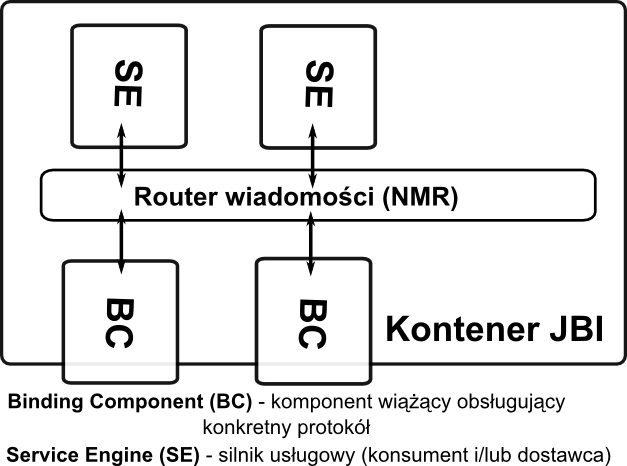
\includegraphics[bb=0 0 300 223]{chapter1/jbi-simple.png}
 % jbi-simple.png: 675x502 pixel, 94dpi, 18.26x13.58 cm, bb=0 0 518 385
 \caption{Nomenklatura JBI\cite{esb:jbi:jbi_components_theory}}
 \label{fig:jbi-simple}
\end{figure}

\paragraph{Jednostka us�ugowa (SU)} (org. service unit) - to jednostka programowa dostarczaj�ca konkretnej implementacji us�ug korzystaj�ca z w�a�ciwo�ci kontenera w kt�rym zosta�a umieszczona. Aplikacje sk�adaj� si� ze skomponowanych SU umieszczonych w kontenerach �rodowiska JBI.

\paragraph{Silniki us�ugowe (SE)} (org. service engine) - to komponenty wykonawcze umieszczane w kontenerze JBI, kt�rych zadaniem jest dostarczanie lub korzystanie z us�ug w jego obr�bie.
Komponenty te dostarczaj� w�a�ciwej logiki takiej jak obs�uga transformacji, regu� biznesowych czy j�zyk�w skryptowych. SE pe�ni� rol� kontener�w dla SU.

\paragraph{Komponenty wi���ce (BC)} (org. binding component) - to komponenty zapewniaj�ce ��czno�� kontenera ze �wiatem zewn�trznym w obu kierunkach - ka�dy z nich realizuje okre�lony protok� komunikacyjny. Wiadomo�ci s� transformowane i przekazywane z i do NMR, kt�ry decyduje o jej dalszej drodze. Takie podej�cie, pozwala ka�demy SE komunikowa� si� ze �wiatem zewn�trznym z pomoc� dowolnego obs�ugiwanego przez kontener protoko�u. Podobnie jak SE, BC r�wnie� pe�ni� rol� kontener�w dla SU.

\paragraph{Router wiadomo�ci o jednolitym formacie (NMR)}(org. Normalized Message Router) -
najwa�niejsza cz�� �rodowiska JBI - stanowi element kt�ry zajmuje si� sterowaniem przep�ywem wiadomo�ci z punkt�w �r�d�owych do punkt�w docelowych, na podstawie okre�lonego z g�ry kontraktu. NMR mo�e r�wnie� realizowa� pewne funkcje QoS dotycz�ce dostarczania wiadomo�ci w obr�bie kontenera.

\paragraph{Kontener JBI} (org. JBI Container) - �rodowisko wykonawcze komponent�w JBI - zar�wno BC jak i SE. 

\subsubsection{Kontrakt}
Implementuj�c komponent JBI, realizujemy pewien kontrakt, kt�ry obejmuje zagadnienia instalacji, pakowania, zarz�dzania cyklem �ycia, publikacji oferowanych us�ugi i przetwarzania wiadomo�ci bazuj�ce na jednym z czterech MEP (Message Exchange Pattern)\footnote{opcjonalnie do kontraktu mo�e nale�e� r�wnie� zarz�dzanie jednostk� us�ugow� (SU - z ang. service unit)}.

\paragraph{MEP - wzorce wymiany wiadomo�ci}
NMR dostarcza wiadomo�ci realizuj�c jeden z czterech wzorc�w wymiany wiadomo�ci b�d�cych cz�ci� specyfikacji WSDL 2.0\cite{ws:wsdl:spec}\cite{esb:sojbi}:

\begin{itemize}
 \item \textbf{In-Only} - standardowy spos�b przesy�ania w jedn� stron�, w kt�rym konsument wysy�a 
 wiadomo�� do dostawcy us�ugi, kt�ry odpowiada statusem 
 \item \textbf{Robust In-Only} - niezawodny spos�b przesy�ania jednokierunkowego, w kt�rym konsument
wysy�a wiadomo�� do dostawcy, kt�ry odpowiada statusem, i je�li jest to b��d (fault), odes�ane zostaje potwierdzenie
 \item \textbf{In-Out} - dwukierunkowy spos�b wymiany wiadomo�ci w kt�rym na wiadomo�� konsumenta,
dostawca us�ugi wysy�a odpowied� kt�ra jest nast�pnie potwierdzana
 \item \textbf{In Optional-Out} - dwukierunkowy spos�b wymiany wiadomo�ci, w kt�rym wiadomo�� b�d�ca 
 odpowiedzi� na ��danie konsumenta jest opcjonalna
\end{itemize}

\subsubsection{Implementacje JBI}
Najszerzej znane implementacje kontenera JBI to:
\begin{itemize}
 \item ServiceMix (FUSE ESB) \cite{esb:impl:servicemix}
 \item OpenJBI (OpenESB) \cite{esb:impl:openesb}
 \item JBossESB \cite{esb:impl:jbossesb}
 \item ObjectWeb2 PEtALS \cite{esb:impl:petals}
\end{itemize}
zgodny z JBI jest r�wnie� MULE \cite{esb:impl:mule}.

Do cel�w pracy wybrano implementacj� OpenJBI firmy Sun Microsystems\texttrademark.

\section{BPEL}
Aby w pe�ni korzysta� z zalet SOA, konieczne jest osi�gniecie niezale�no�ci kompozycji us�ug, od ich implementacji.\cite{bpel:book:bpel4ws}

Istniej� dwa podej�cia do tego zagadnienia \cite{bpel:book:wsbpel}:
\begin{itemize}
 \item \textbf{Orchiestracja} - w kt�rej jeden centralny komponent przejmuje kontrol� nad us�ugami 
 b�d�cymi uczestnikami procesu biznesowego, koordynuj�c ich wsp�prac�. Us�ugi nie s� �wiadome bycia
  uczestnikami procesu biznesowego (przyk�ad ilustruje rys \ref{fig:bpel_orchiestracja}).
  \begin{figure}[h!tb]
   \centering
   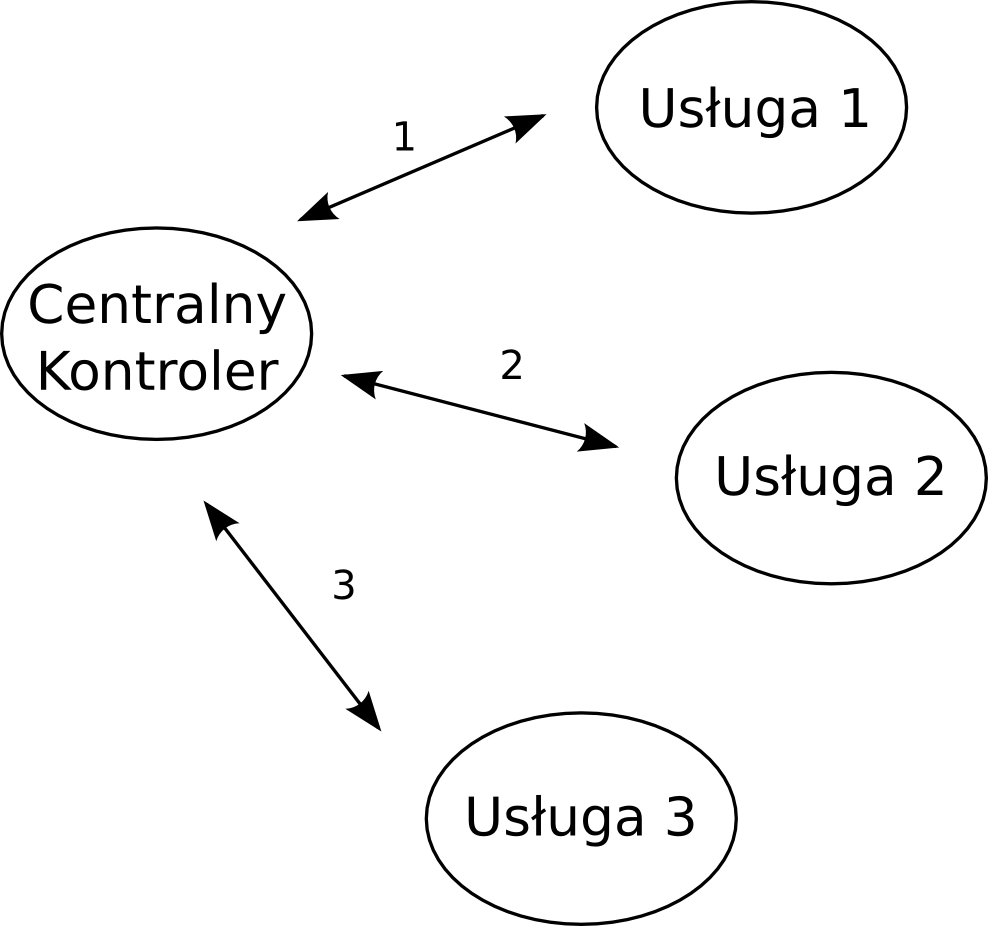
\includegraphics[bb=0 0 237 222]{chapter1/orchiestracja.png}
   % orchiestracja.png: 306x287 pixel, 93dpi, 8.36x7.84 cm, bb=0 0 237 222
   %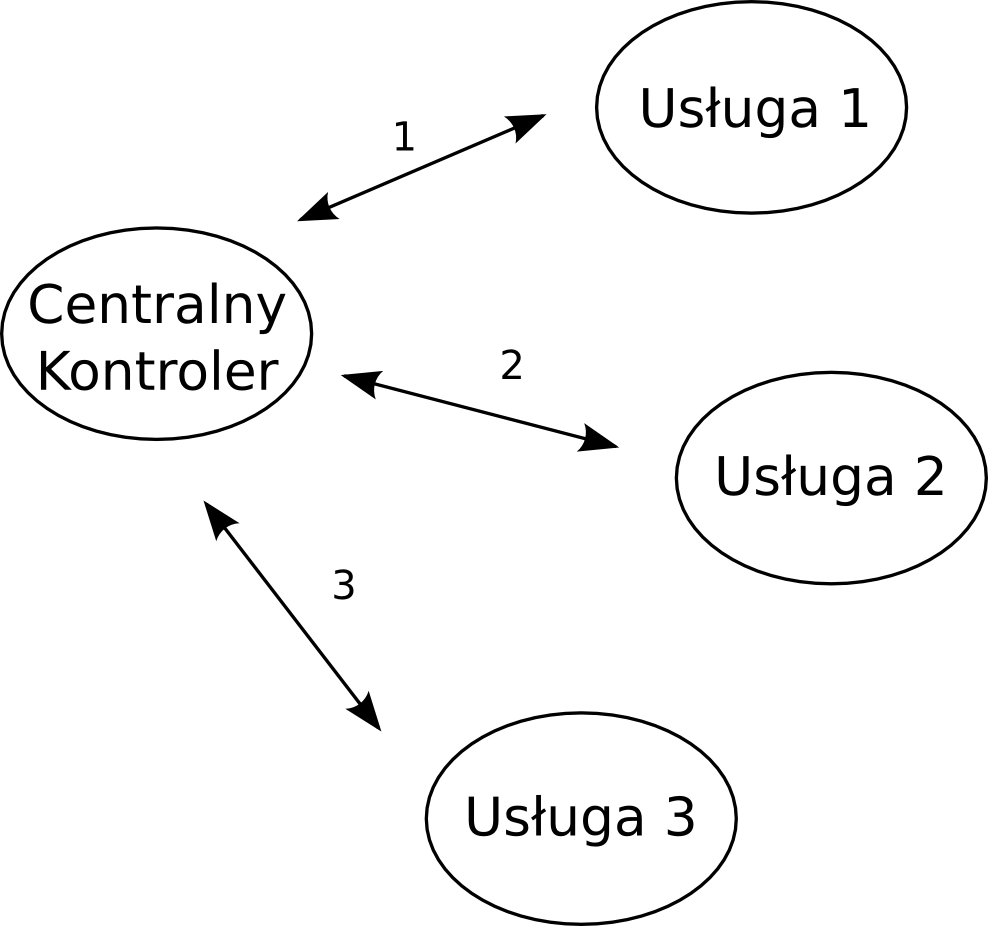
\includegraphics[bb=0 0 311 238]{chapter1/orchiestracja.png}
   %% orchiestracja.png: 384x294 pixel, 89dpi, 10.96x8.39 cm, bb=0 0 311 238
   \caption{Orchiestracja}
   \label{fig:bpel_orchiestracja}
  \end{figure}

 \item \textbf{Choreografia} - podej�cie w kt�rym zamiast jednego centralnego punktu, ka�da us�uga wie
kiedy i z jakimi us�ugami ma si� komunikowa�. Us�ugi musz� by� �wiadome uczestniczenia w procesie biznesowym (przyk�ad ilustruje rysunek \ref{fig:bpel_choreografia}).
\begin{figure}[htb!]
 \centering
 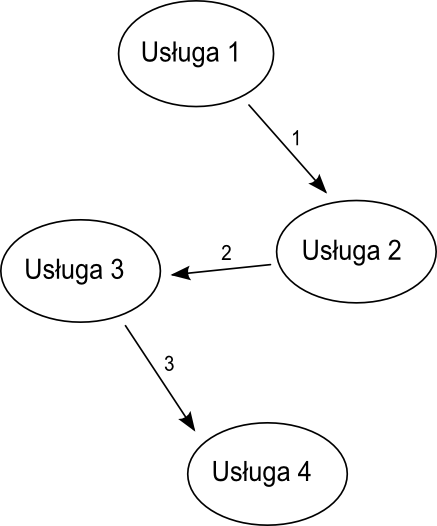
\includegraphics[bb=0 0 210 252]{chapter1/choreografia.png}
 % choreografia.png: 271x326 pixel, 93dpi, 7.40x8.90 cm, bb=0 0 210 252
 %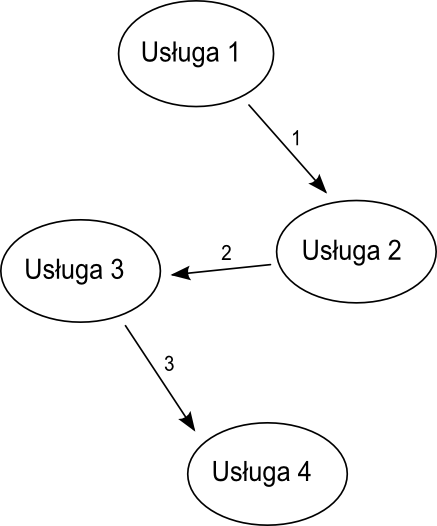
\includegraphics[bb=0 0 211 254]{chapter1/choreografia.png}
 % choreografia.png: 609x422 pixel, 93dpi, 16.63x11.53 cm, bb=0 0 472 327
 \caption{Choreografia}
 \label{fig:bpel_choreografia}
\end{figure}

\end{itemize}



% mo�e jaki� krotki tekst o tym ze �eby w pe�ni korzystac z SOA musimy jako� osi�gn�� kompozycje us�ug, i tu ew wymieni� podej�cie orchiestracji i choreografii, nastepnie napisa� o BPEL.
% Powstanie j�zyka BPEL mia�o zwi�zek z potrzeb� oddzielenia logiki element�w procesu od jego przebiegu.

% kr�tko wspomnie� o tym kto mia� wp�yw na powstanie j�zyka, 

\textbf{BPEL}\cite{bpel:spec} (Business Process Execution Language) jest to zdefiniowany przez organizacj� OASIS j�zyk orchiestracji proces�w biznesowych opartych o us�ugi zdefiniowane w j�zyku WSDL.

J�zyk ten pozwala na modelowanie na dw�ch poziomach abstrakcji: opisowym poziomie abstrakcyjnym(z ang. Abstract Business Process)\footnote{modele takie nie maj� by� wykonywane, a s� jedynie tworzone celem zobrazowania pewnego konkretnego procesu} i dok�adniejszym poziomie wykonania(z ang. Executable Business Process)\cite{bpel:spec}.

Interakcja z us�ugami w j�zyku BPEL odbywa si� na dwa sposoby:
\begin{itemize}
 \item eksport funkcjonalno�ci, wykonanie procesu BPEL jest zwykle wyzwalane poprzez ��danie wykonania operacji webservice
 \item import funkcjonalno�ci, proces BPEL umo�liwia wykonanie operacji na us�ugach webservice
\end{itemize}

\subsection{Wersje BPEL}

\paragraph{Wersje 1.0 i 1.1}
BPEL,a w zasadzie BPEL4WS (Business Process Execution Language for Web Services) powsta� w 2002 jako efekt wsp�pracy firm BEA, IBM i Microsoft. W roku 2003 do organizacji specyfikuj�cej BPEL do��czy�y firmy SAP oraz Siebel Systems, a j�zyk ewoluowa� do wersji 1.1. Wersja ta zosta�a zaaprobowana przez organizacj� OASIS (Organization for the Advancement of Structured Information Standards), i od tamtego czasu j�zyk ten sta� si� standardem w dziedzinie kompozycji proces�w biznesowych\cite{bpel:bpeljava}\cite{bpel:book:wsbpel}\cite{bpel:wikipedia}\cite{bpel:spec1.1}.

\subparagraph{Mo�liwo�ci j�zyka BPEL w wersji 1.1}
Specyfikacja j�zyka BPEL przewiduje nast�puj�ce mo�liwo�ci:

\begin{itemize}
 \item definiowanie typowanych zmiennych i synchronizowany dost�p do nich
 \item wykonywanie operacji webservice
 \item r�wnoleg�e wykonywanie operacji 
 \item definiowanie zasi�g�w (scope) dla zmiennych
 \item rzucanie i obs�ugiwanie wyj�tk�w
 \item dost�p do zmiennych za pomoc� wyra�e� XPath
 \item manipulacja zmiennymi
\end{itemize}

% ci�ko powiedziec co tu wstawi�

\subparagraph{Dost�pne konstrukcje} BPEL w wersji 1.1 oferuje nast�puj�ce konstrukcje:
\begin{itemize}
 \item \textbf{Proste}
 \begin{itemize}
  \item \textbf{Assign} przypisanie warto�ci zmiennej
  \item \textbf{Wait} oczekiwanie okre�lony okres czasu
  \item \textbf{Empty} instrukcja pusta
  \item \textbf{Throw} rzucenie wyj�tku
  \item \textbf{ReThrow} ponowne rzucenie z�apanego wyj�tku
  \item \textbf{Exit} zako�czenie procesu				 
  \item \textbf{Compensate} pozwalaj�ce na zdefiniowanie zachowania procesu w obr�bie transakcji, w przypadku, gdy jedna z jego sk�adowych zawiedzie (pr�ba odwr�cenia efekt�w dzia�ania element�w ju� wykonanych\footnote{analogiczne do zachowania transakcyjno�ci w bazach danych, tzw. ACID (skr�t ten pochodzi z terminologii baz danych, i oznacza cztery warunki jakie musz� spe�nia� transakcje: atomowo��, sp�jno��, izolacja i trwa�o�� (z ang. Atomicity, Consistency, Isolation, Durability)\cite{bpel:acid})})
 \end{itemize}
 \item \textbf{Strukturalne}
 \begin{itemize}
    \item \textbf{Sequence} wydzielony blok strukturalny
    \item \textbf{Scope} zasi�g zmiennej
    \item \textbf{If} instrukcja warunkowa
    \item \textbf{While} p�tla z warunkiem ewaluowanym na jej pocz�tku
    \item \textbf{Pick} oczekiwanie na jedno z zadeklarowanych zdarze�
    \item \textbf{Flow} wykonanie r�wnoleg�e
  \end{itemize}
  \item \textbf{Operacje na us�ugach webservice}
  \begin{itemize}
    \item \textbf{Receive} odebranie wiadomo�ci z us�ugi dostarczanej przez
     proces\footnote{operacja ta jest najcz�ciej operacj� wyzwalaj�c� proces}
    \item \textbf{Reply} odpowied� na odebran� wiadomo��\footnote{analogicznie
     operacja taka najcz�ciej ko�czy wyzwolony proces}
    \item \textbf{Invoke} wykonanie operacji na us�udze webservice.
  \end{itemize}
\end{itemize}


\subsubsection{Wersja 2.0}
Opracowana w roku 2004 nowa wersja j�zyka BPEL wprowadzi�a takie usprawnienia jak mo�liwo�� rozszerzania j�zyka, czy uproszczenia w przypisywaniu i inicjalizacji zmiennych. Pojawi�y si� nowe p�tle: RepeatUntil\footnote{p�tla z warunkiem ewaluowanym na jej ko�cu} i wykonywana zar�wno r�wnolegle, jak i sekwencyjnie ForEach\footnote{p�tla dokonuj�ca pewnych operacji na zbiorze danych}. Uproszczono r�wnie� obs�ug� b��d�w oraz inicjalizacj� tzw. Partner Link\footnote{odniesie� do us�ug w obr�bie proces�w}. Zmieniono r�wnie� oficjaln� nazw� j�zyka - obecnie oficjaln� nazw� jest WS-BPEL (Web Service - Business Process Execution Language)\footnote{uczyniono tak celem dopasowania si� do pozosta�ych nazw standard�w z zakresu technologii webservice kt�rych nazwy zwyczajowo zaczynaj� si� od ``WS-''}\cite{bpel:bpeljava}\cite{bpel:book:wsbpel}\cite{bpel:wikipedia}\cite{bpel:spec2}. \\
\\
Wszystkie dost�pne obecnie konstrukcje j�zyka BPEL, wraz z ich graficznymi reprezentacjami przedstawia rysunek \ref{fig:bpel_pallette}(nale�y mie� jednak na uwadze fakt, i� reprezentacje te nie stanowi� cz�ci standardu).

% \begin{figure}[h!tb]
%  \centering
%  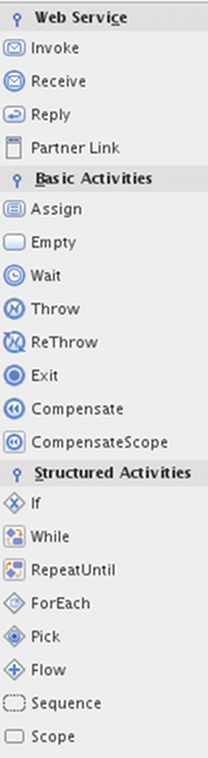
\includegraphics[width=200pt,bb=0 0 373 230]{chapter1/netbeans_pallette.png}
%  % netbeans_pallette.png: 373x230 pixel, 72dpi, 13.16x8.11 cm, bb=0 0 373 230
%  \caption{Elementy konstrukcyjne j�zyka BPEL}
%   \label{fig:bpel_pallette} 
% \end{figure}

\begin{figure}[h!kp]
 \centering
 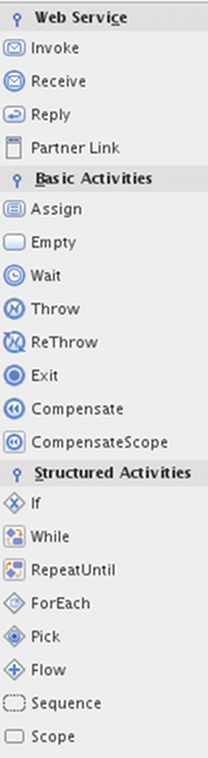
\includegraphics[bb=0 0 100 363]{chapter1/netbeans_pallette.png}
 % netbeans_pallette.png: 162x548 pixel, 72dpi, 5.71x19.33 cm, bb=0 0 162 548
 \caption{Elementy konstrukcyjne j�zyka BPEL}
 \label{fig:bpel_pallette}
\end{figure}



% \begin{figure}[htb]
%  \centering
%  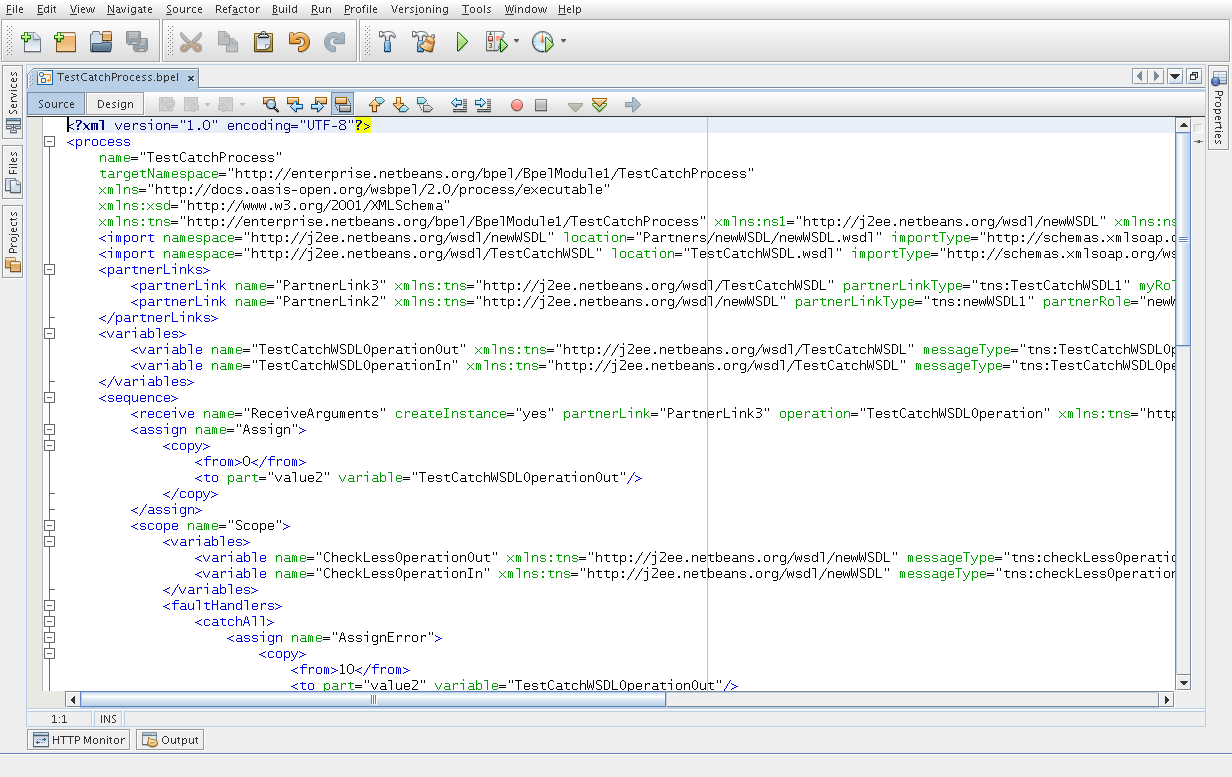
\includegraphics[width=12cm,height=8cm,bb=0 0 1232 777]{chapter1/bpel_src.png}
%  % bpel_src.png: 1232x777 pixel, 72dpi, 43.47x27.42 cm, bb=0 0 1232 777
%  \caption{Pakiet NetBeans - proces BPEL opisany w XML}
%  \label{fig:bpel_sample_src}
% \end{figure}

\subsection{Dost�pne implementacje BPEL}
J�zyk BPEL jest obs�ugiwany w wielu �rodowiskach integracyjnych, zar�wno jako komponenty, jak i samodzielne rozwi�zania. Do najbardziej rozwini�tych komercyjnych rozwi�za� nale��\cite{bpel:book:bpel4ws}:
\begin{itemize}
 \item IBM Websphere Business Integration Foundation\texttrademark\cite{esb:impl:websphere}
 \item Oracle BPEL Process Manager\texttrademark\cite{bpel:impl:oracle}
 \item Microsoft BizTalk\texttrademark\cite{bpel:impl:biztalk}
 \item BEA Aqualogic\texttrademark\cite{esb:impl:aqualogic}
\end{itemize}

Istnieje r�wnie� kilka rozwi�za� niekomercyjnych takich jak:
\begin{itemize}
 \item OpenESB BPEL JBI Component\cite{esb:impl:openesb}
 \item ActiveBPEL Engine\cite{bpel:impl:activebpel}
 \item Apache ODE\cite{bpel:impl:ode}
\end{itemize}

\begin{figure}[h!kp]
 \centering
 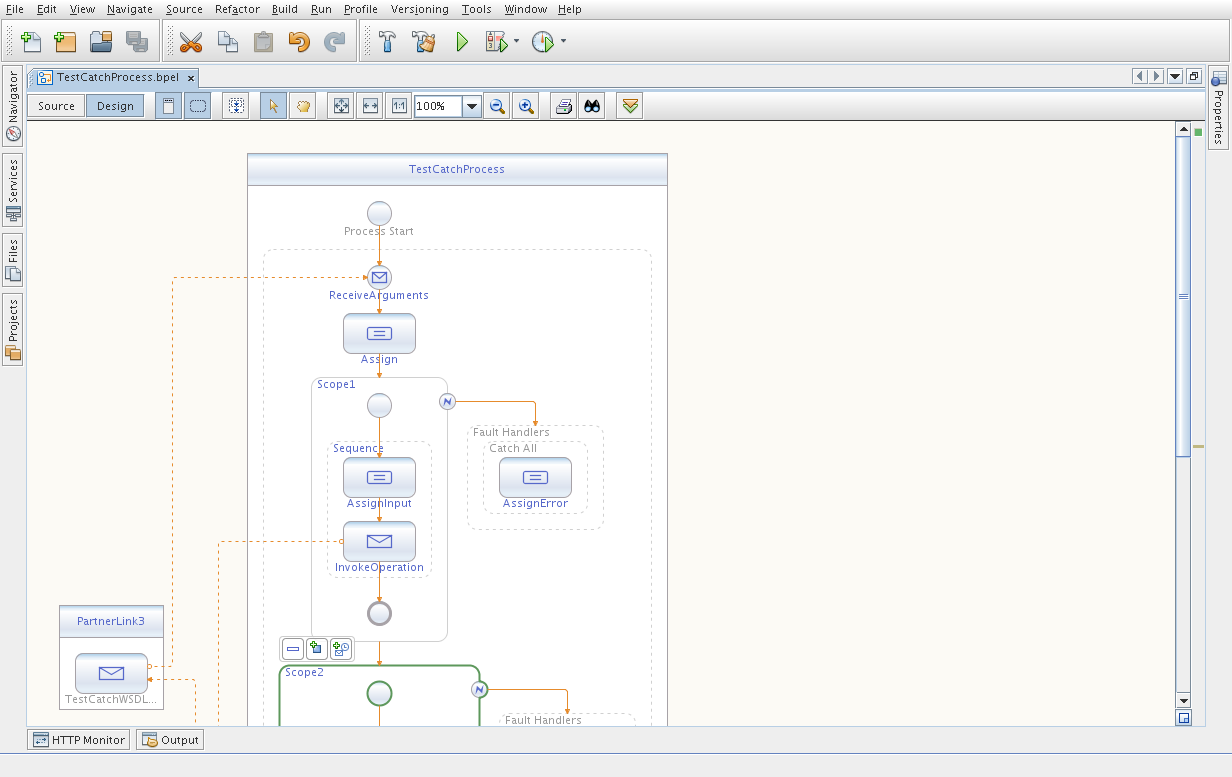
\includegraphics[width=12cm,height=8cm,bb=0 0 1232 777]{chapter1/bpel_des.png}
 % bpel_des.png: 1232x777 pixel, 72dpi, 43.47x27.42 cm, bb=0 0 1232 777
 \caption{Pakiet Netbeans - wizualny edytor procesu BPEL}
 \label{fig:bpel_sample_des}
\end{figure}

Istnieje r�wnie� szereg narz�dzi u�atwiaj�cych modelowanie proces�w w j�zyku BPEL, takich jak oparte na platformie Eclipse Oracle BPEL Designer\cite{bpel:tool:oracle} i IBM Websphere Application Developer Integration Edition\cite{bpel:tool:websphere}, czy wybrany przez autor�w, oparty o platform� Netbeans BPEL Designer\cite{bpel:tool:netbeans} (przedstawiony na rys. \ref{fig:bpel_sample_des}). Wyb�r ten zosta� podyktowany dojrza�o�ci� i otwarto�ci� rozwi�zania, oraz zaawansowan� integracj� z wybranym wcze�niej �rodowiskiem OpenESB.


\newpage

Wysoka innowacyjno�� opisanych w niniejszym rozdziale koncepcji i technologii, sprawia �e nie s� one obecnie w powszechnym u�yciu.
% Opisane w niniejszym rozdziale koncepcje i technologie stanowi� innowacyjne rozwi�zania, nie b�d�ce jeszcze w powszechnym u�yciu w �wiecie oprogramowania du�ej skali.
Wydajno�� aplikacji zrealizowanych z ich u�yciem, mo�e by� badana z u�yciem oprogramowania stworzonego w ramach niniejszej pracy.
% Aplikacje stworzone z ich pomoc� s� przedmiotem test�w stworzonego w ramach pracy oprogramowania.